\documentclass[conference]{IEEEtran}
\IEEEoverridecommandlockouts
% The preceding line is only needed to identify funding in the first footnote. If that is unneeded, please comment it out.
\usepackage{cite}
\usepackage{amsmath,amssymb,amsfonts}
\usepackage{algorithmic}
\usepackage{graphicx}
\usepackage{textcomp}
\usepackage{xcolor}
\graphicspath{{Images/}}
\def\BibTeX{{\rm B\kern-.05em{\sc i\kern-.025em b}\kern-.08em
    T\kern-.1667em\lower.7ex\hbox{E}\kern-.125emX}}

\renewcommand*\descriptionlabel[1]{\hspace\leftmargin$#1$}

\begin{document}
\title{SVD Implementation on MNIST Image Classification Based on CNN\\
}

\author{\IEEEauthorblockN{Satrya Budi Pratama}
\IEEEauthorblockA{\textit{Institut Teknologi Bandung} \\
\textit{Sekolah Teknik Elektro dan Informatika}\\
Bandung, Indonesia \\
satrya@zeroinside.net}
}

\maketitle

\begin{abstract}
In recent years, many development has been made in the field of image classification. Deep learning has proven to be powerful for classficiation, one of them is convolutional neural networks (CNN). 
In image classification one of the challange is to recognized the handwritten digit. 
CNN architecture which has high precision for that problem is Lenet-5.

In this paper, we recognized the handwritten of MNIST dataset and implement SVD for feature extraction as preprocessing method. 
We build LeNet-5 model and evaluate the model. 
\end{abstract}

\begin{IEEEkeywords}
CNN, LeNet-5, SVD, MNIST
\end{IEEEkeywords}

\section{Introduction}
Handwriting recognition is the recognition of handwritten letters, numbers and symbols by computer systems \cite{maad2015}.
The problem is every handwritten has different style. 
Every person has their style of writting a character, word and symbol. 
The computer try to assign the digitilzed character to its symbolic class. 
In the case of a print image, this is referred to as optical character recognition (OCR) 
meanwhile in the case of handprint, it is loosely referred to as intelligent character recognition (ICR) \cite{824821}.
This has been a topic of research for decades. 
Some of the research areas include signature verification, bank check processing, postal address interpretation from envelopes, and get the digits on test letter for recuirement.

In recent years, the rise of artificial intelligent (AI) and big data especially in machine learning has brought a rapid
development in the handwriting recognition application. 
Google has been developed Vision AI \footnote{https://developers.google.com/ml-kit/vision} that can be used for reading printed and handwritten text. 
Some mobile application also has the OCR features such as Pen to Print \footnote{https://www.pen-to-print.com},
Notes Plus \footnote{https://new.notesplusapp.com/}, and
Photomath \footnote{https://photomath.net}. The web application such as i2OCR \footnote{http://www.i2ocr.com/about}, OnlineOCR \footnote{https://www.onlineocr.net/},
and Convertio\footnote{https://convertio.co/ocr/}. All of these technologies are use machine learning for the recognition or classificaion model. 

Deep learning is one of the popular method on machine learning. It has been highly and widely implemented in various research fields especially in image recognition.
The most important property of deep learning methods is that it can automatically learn feature representations thus avoiding a lot of time-consuming engineering \cite{musab2017deep}.
Betterchip processing abilities, considerable advances in the machine learning algorithms, and affordable cost of computing hardware are primarily crucial reasons for the booming of deep learning \cite{lecun2015deep}.

One of them is Convolutional Neural Network (CNN). CNN  was firstly  introduced  by Kunihiko  Fukushima  \cite{fukushima1980neocognitron}. It  was  later proposed  by  Yann 
LeCun.  He  combined  CNN  with  back-propagation  theory  to  recognize  handwritten  digits  and 
document recognition \cite{lecun1990handwritten,lenet-5}. His system called LeNet-5, it was eventually used to read hand-written checks and zip codes.
CNN is a powerful technique for image processing as well as natural language processing. 
The main advantage of CNN is the high accuracy in its results. However, it requires high computational cost. 
In addition, it needs a lot of data to be trained. The complexity of the CNN slows down the training process thus it is necessary to use a good GPU to overcome this problem \cite{alsaafin2017minimal}.
Beside the hardware, another approach to reduce computational cost by eliminating the features as input to the model and use low-rank approximation. 
Liu et al. \cite{liu2008classification} claim that training classifiers using MNIST dataset without using feature extraction methods shows inferior performance.
This motivates us to use SVD as feature extraction and compare the performance to its original features from MNIST dataset using LeNet-5 model. 

\section{Dataset and SVD}

\subsection{MNIST Dataset}
In this paper, we use Modified National Institute of Standards and Technology (MNIST) dataset. 
The MNIST is a dataset developed by LeCun, Cortes, and Burges for evaluating machine learning models on the handwritten digit classification problem \cite{lenet-5}. 
It has been widely used in research and to design novel handwritten digit recognition systems. 
It contains $60,000$ training cases and $10,000$ test cases of handwritten digits (0 to 9). 
Each digit is normalized and centered in a gray-scale (0 - 255) image with dimension $28 \times 28$. 
Each image consists of $784$ pixels that represent the features of the digits. An example of a digit can be shown in \ref{fig:sevenMNIST} and a example of dataset in \ref{fig:100mnist}. 

\begin{figure}[htbp]
    \centerline{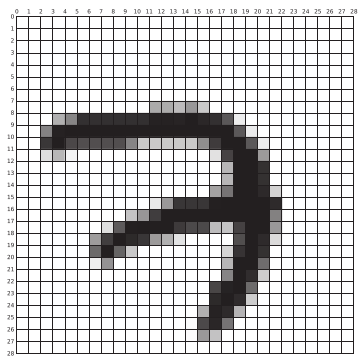
\includegraphics[width=8cm]{detail7.png}}
    \caption{MNIST sample belonging to the digit 7 adopted from \protect\cite{baldominos2019survey}}
    \label{fig:sevenMNIST}
\end{figure}

\begin{figure}[htbp]
    \centerline{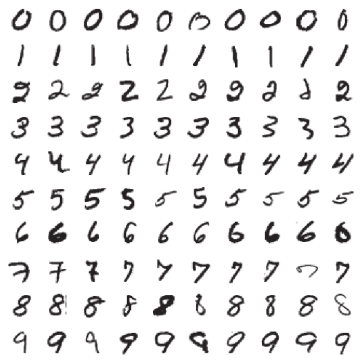
\includegraphics[width=8cm]{100MNIST.png}}
    \caption{100 digit example of a MNIST dataset adopted from \protect\cite{baldominos2019survey} }
    \label{fig:100mnist}
\end{figure}

\subsection{SVD}
Singular Value Decomposition or SVD intimately related to the familiar theory of diagonalizing a symmetric matrix \cite{kalman1996singularly}. 
SVD says that rectangular matrix A can be broken down into the product of three matrices : an orthogonal matrix U, a diagonal matrix $\Sigma$, and the transpose of an orthogonal matrix V as equation \ref{eq:SVD} below.
\begin{equation}
    \label{eq:SVD}
    A_{m \times n} = U_{m\times m} \Sigma_{m\times n} V_{n\times n}^T
\end{equation}
where : 
\begin{description}
    \item[$U^TU$] : Identity Matrix (I)
    \item[$V^TV$] : Identity Matrix (I)
    \item[$U$] : orthonormal eigenvectors of $AA^T$
    \item[$V$] : orthonormal eigenvectors of $A^TA$
    \item[$\Sigma$] : diagonal matrix containing the square roots of eigen values from U or V in descending order.  
\end{description}

SVD is a method for identifying and ordering the dimensions
along which data points exhibit the most variation. This ties in to the third way of viewing
SVD, which is that once we have identified where the most variation is, it’s possible to find
the best approximation of the original data points using fewer dimensions. Hence, SVD can
be seen as a method for data reduction. Also the SVD applied on linear squares optimization and data compression with reduced rank approximation on \cite{kalman1996singularly}.

To construct matrix with the low-rank approximation obtain from SVD, with the number of components as $k$ in \ref{eq:low_rank_SVD}.
\begin{equation}
    \label{eq:low_rank_SVD}
    A_{m \times n} = U_{m\times k} \Sigma_{k\times k} V_{k\times n}^T 
\end{equation}


\section{Implementation}
We use LeNet-5 architecture to train model on MNIST dataset using TensorFlow. The architecture of the networks shown in \ref{fig:lenet-5archi}.
\begin{figure}[htbp]
    \centerline{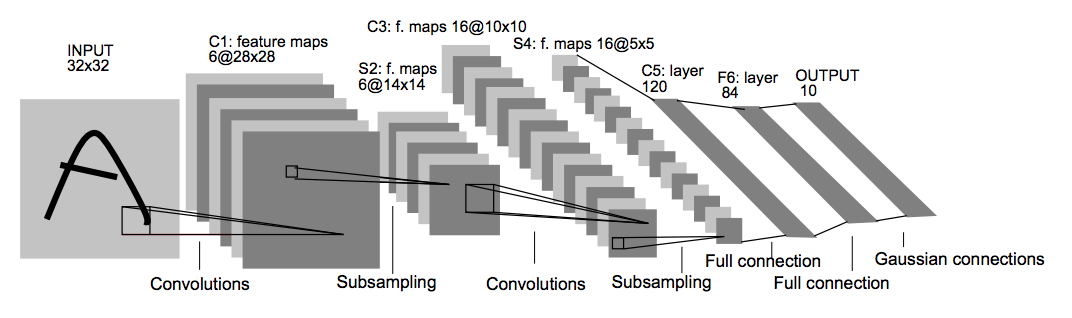
\includegraphics[width=9cm]{LeNet-5Architecture.png}}
    \caption{LeNet-5 Architecture adopted from \protect\cite{lenet-5} }
    \label{fig:lenet-5archi}
\end{figure}
It has 7 layers exclude the input layer, it's basicaly consist of convolutional layer, pooling layer, and fully connection layer.
\begin{enumerate}
    \item Convolution

    This layer has input dimension $32 \times 32 \times 1$ and the output is $28 \times 28 \times 6$.
    We will use ReLu activation function since it's better than sigmoid \cite{wang2020improvement}.

    \item Subsampling or Pooling 
    
    This layer has input dimension $28 \times 28 \times 6$ and the output is $14 \times 14 \times 6$.

    \item Convolution
    
    This layer has input dimension $14 \times 14 \times 6$ and the output is $10 \times 10 \times 16$. Also has ReLu activation function.

    \item Subsampling or Pooling 
    
    This layer has input dimension $10 \times 10 \times 16$ and the output is $5 \times 5 \times 16$.

    \item Fully Connected
    
    This layer has input dimension $5 \times 5 \times 16$ and the output is $120$.

    \item Fully Connected
    
    This layer has input dimension $120$ and the output is $84$.

    \item Output  
    
    This layer has input dimension $84$ and the output is $10$.

\end{enumerate}
As suggestion by Wang et al \cite{wang2020improvement}, to imporve the LeNet-5 model on MNIST dataset is to use $0.0002$ learning rate and add drop out layer before output layer.
So we use Adam as optimizer with $0.0002$ learning rate, and add $0.2$ dropout layer before output layer.

First step was downloaded the MNIST dataset \footnote{http://yann.lecun.com/exdb/mnist/}. There are 4 main file for training data and testing data.
The training data contains $60,000$ examples, and the testing data $10,000$ examples.
However, the LeNet-5 architecture only accepts 32x32xC images, where C is the number of color channels. 
In order to reformat the MNIST data into a shape that LeNet-5 will accept, we pad the data with $n$ rows of zeros on the top and bottom, and $n$ columns of zeros on the left and right. 
The number of $n$ is a half of substraction between $32$ and feature extraction dimension. The original MNIST has $28 \times 28$ so we pad 2 rows at top and bottom, then 2 columns on left and right.

Before train the model, we did several preprocessing method. We shuffled the dataset and splited training data into 2 sets: $20 \%$ train (48,000 images) and $80 \%$ validation (12,000 images).
We applied SVD as feature extraction to all data, with the $k$ number of components. We will choose $k$ in range $2, 4, 6, ..., 30$ based on the highest accuracy of evaluate model.

We trained the model with 12 epoch with SVD and without SVD using training data and validation data. We tested the model using testing data and evalutate both model then compared the performance between two method.
\section{Result and Analysis}
\subsection{Preprocessing with SVD}
We compared the sample images from MNIST and the result of the preprocessing data. 
The result between the original features of the images can be shown in \ref{fig:original_img}, and the reconstructed image with 2 number of components can be shown in \ref{fig:svd_2_comp}.
\begin{figure}[htbp]
    \centerline{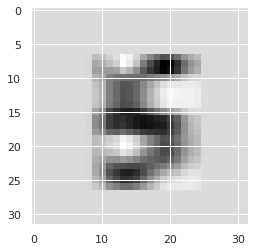
\includegraphics[width=4cm]{SVD_2_comp.png}}
    \caption{Reconstructed Sample Image }
    \label{fig:svd_2_comp}
\end{figure}
\begin{figure}[htbp]
    \centerline{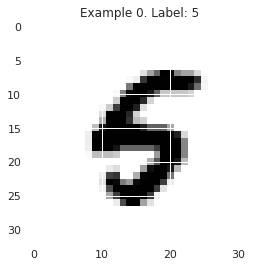
\includegraphics[width=4cm]{raw_image.png}}
    \caption{Original MNIST Sample Image}
    \label{fig:original_img}
\end{figure}
It gives the blurry images with lower number of components, and more detail with higher number of components. It's just has reduced rank of the matrix, 
so the value of the pixels is lower than before. The image dimension also not reduced, it stays with $32\times32$ since we don't use principal components analysis (PCA) approach but low-rank approximation.  

\subsection{Training Model}
We trained the model with original data and SVD data. As we used the validation data, we can test the trained model on every epoch and give the performance.
The accuracy without SVD can be shown in \ref{fig:trained_model_without_SVD} and the accuracy with SVD can be shown in \ref{fig:trained_model_with_SVD}
\begin{figure}[htbp]
    \centerline{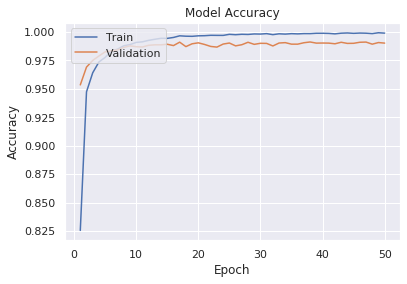
\includegraphics[width=7cm]{Training_performance_acc.png}}
    \caption{Accuracy of Trained Model without SVD}
    \label{fig:trained_model_without_SVD}
\end{figure}

\begin{figure}[htbp]
    \centerline{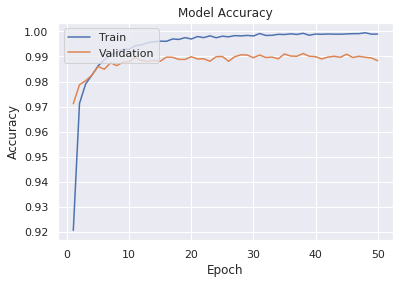
\includegraphics[width=7cm]{Training_performance_SVD_acc.png}}
    \caption{Accuracy of Trained Model with SVD}
    \label{fig:trained_model_with_SVD}
\end{figure}
We focused on validation data not on the training data itself, since training data had been seen by our model.
The highest validation accuracy is $99.09 \%$ until 11 epoch on model without SVD, and $99.17 \%$ until 12 epoch on model with SVD. 
So, we can choose the best model according to the epoch. From the result, we can conclude that SVD model gives higher accuracy.  

\subsection{Testing Model}
We tested the model with data testing without SVD and with SVD.  

\section*{Acknowledgment}

The preferred spelling of the word ``acknowledgment'' in America is without 
an ``e'' after the ``g''. Avoid the stilted expression ``one of us (R. B. 
G.) thanks $\ldots$''. Instead, try ``R. B. G. thanks$\ldots$''. Put sponsor 
acknowledgments in the unnumbered footnote on the first page.
\cite{{wang2020improvement}}

\bibliographystyle{IEEEtran}
\bibliography{IEEEabrv,References}


\end{document}
